%!TEX root = ../GLM_Becerra_Lopez.tex

\section*{Apéndice: convergencia de cadenas}
\label{sec:appendix}


\subsection*{Modelo de unidades iguales}

\begin{figure}[H]
    \centering
    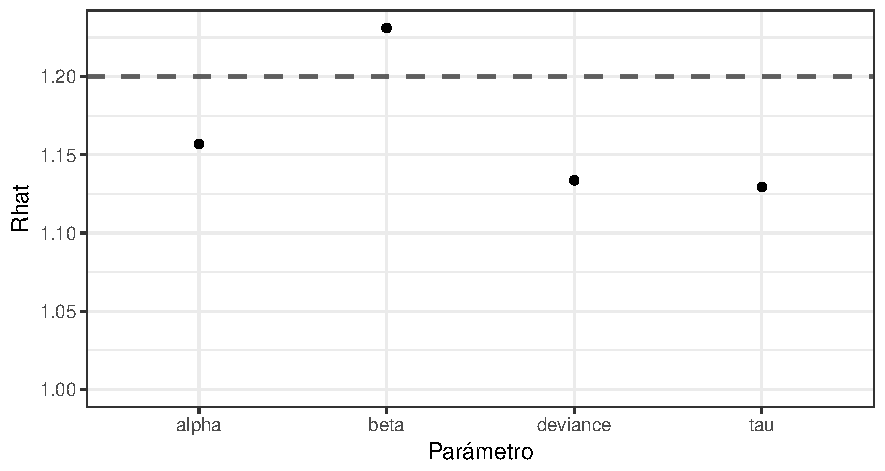
\includegraphics[width=0.9\textwidth]{images/comp_pooling_r_statistic_params.pdf}
    \caption{Estadística de convergencia $\hat{R}$ de Gelman y Rubin para cada parámetro del modelo de unidades iguales}
    \label{fig:comp_pooling_r_statistic_params}
\end{figure}

\begin{figure}[H]
    \centering
    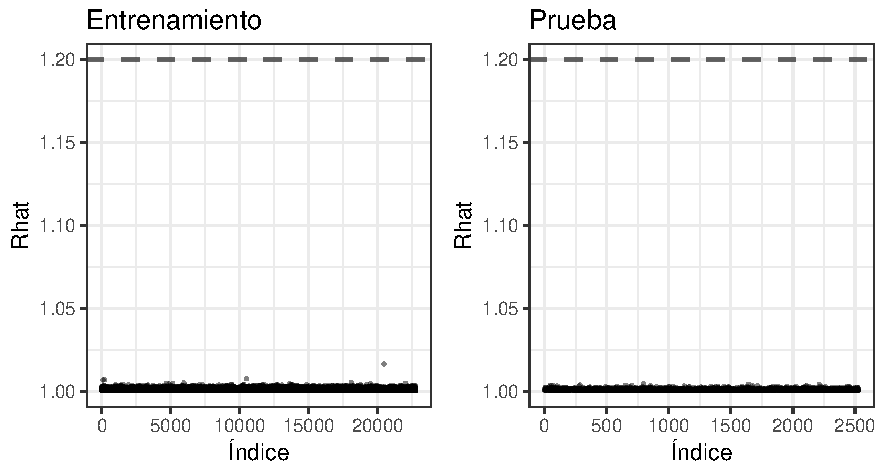
\includegraphics[width=0.9\textwidth]{images/comp_pooling_r_statistic_yf.pdf}
    \caption{Estadística de convergencia $\hat{R}$ de Gelman y Rubin para estimaciones de la variable respuesta del modelo de unidades iguales}
    \label{fig:comp_pooling_r_statistic_yf}
\end{figure}

\begin{figure}[H]
    \centering
    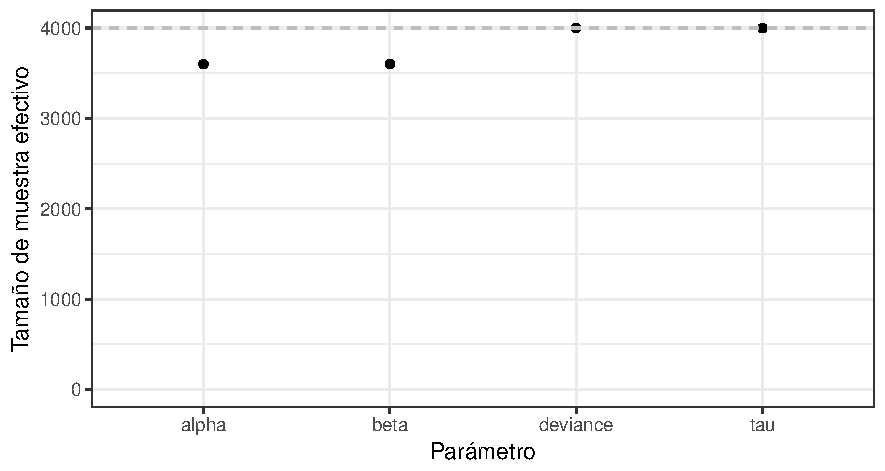
\includegraphics[width=0.9\textwidth]{images/comp_pooling_n_eff_params.pdf}
    \caption{Tamaño de muestra efectivo para cada parámetro del modelo de unidades iguales}
    \label{fig:comp_pooling_n_eff_params}
\end{figure}

\begin{figure}[H]
    \centering
    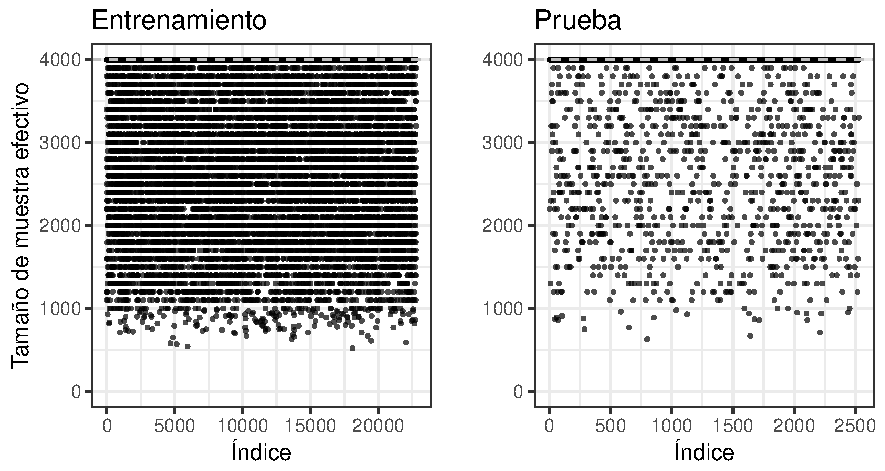
\includegraphics[width=0.9\textwidth]{images/comp_pooling_n_eff_yf.pdf}
    \caption{Tamaño de muestra efectivo para cada estimación de la variable respuesta del modelo de unidades iguales}
    \label{fig:comp_pooling_n_eff_yf}
\end{figure}



\subsection*{Modelo de unidades independientes}

\begin{figure}[H]
    \centering
    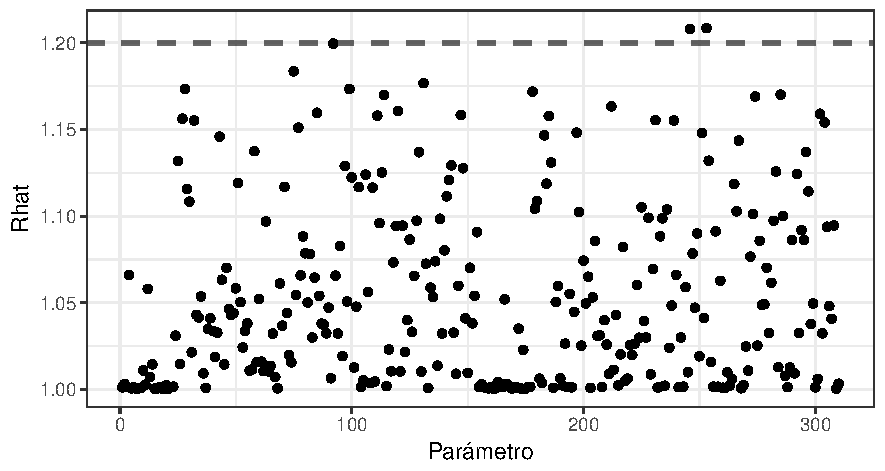
\includegraphics[width=0.9\textwidth]{images/no_pooling_r_statistic_params.pdf}
    \caption{Estadística de convergencia $\hat{R}$ de Gelman y Rubin para cada parámetro del modelo de unidades independientes}
    \label{fig:no_pooling_r_statistic_params}
\end{figure}

\begin{figure}[H]
    \centering
    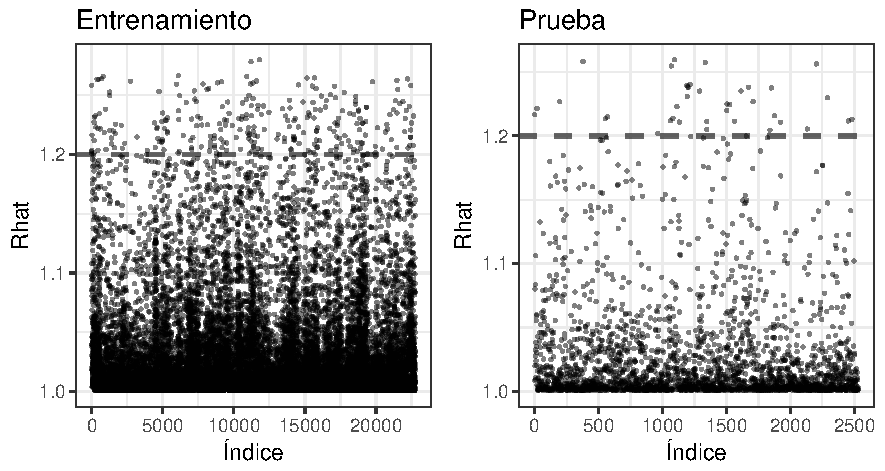
\includegraphics[width=0.9\textwidth]{images/no_pooling_r_statistic_yf.pdf}
    \caption{Estadística de convergencia $\hat{R}$ de Gelman y Rubin para estimaciones de la variable respuesta del modelo de unidades independientes}
    \label{fig:no_pooling_r_statistic_yf}
\end{figure}

\begin{figure}[H]
    \centering
    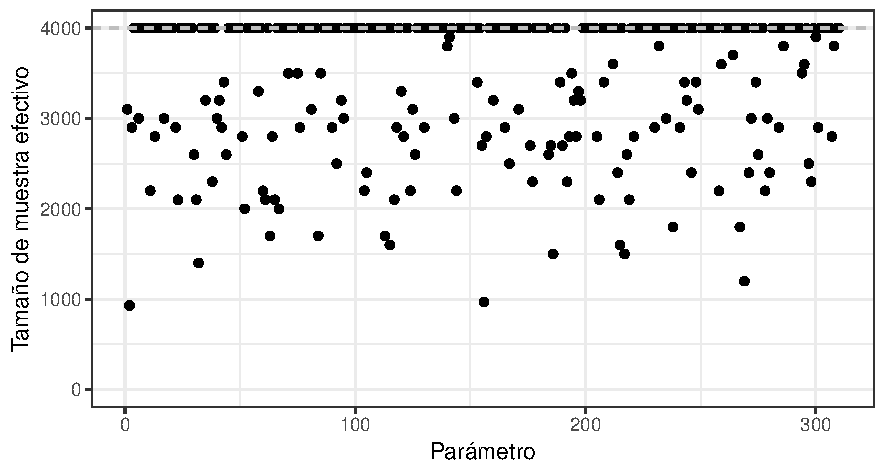
\includegraphics[width=0.9\textwidth]{images/no_pooling_n_eff_params.pdf}
    \caption{Tamaño de muestra efectivo para cada parámetro del modelo de unidades independientes}
    \label{fig:no_pooling_n_eff_params}
\end{figure}

\begin{figure}[H]
    \centering
    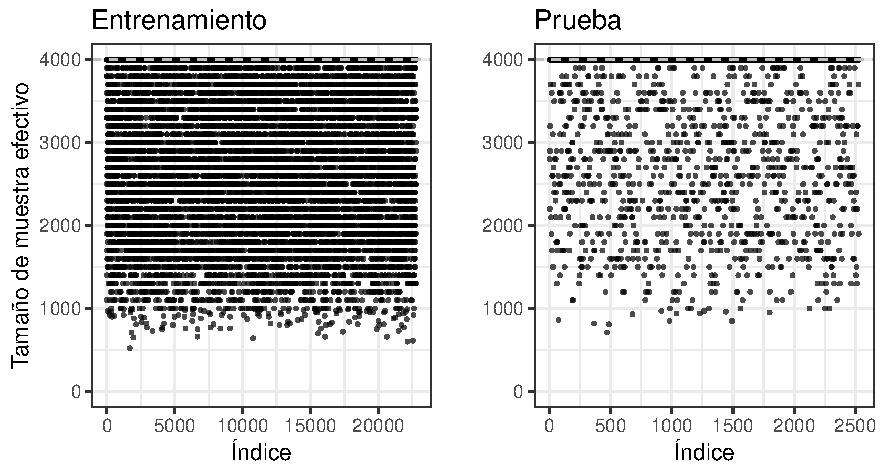
\includegraphics[width=0.9\textwidth]{images/no_pooling_n_eff_yf.pdf}
    \caption{Tamaño de muestra efectivo para cada estimación de la variable respuesta del modelo de unidades independientes}
    \label{fig:no_pooling_n_eff_yf}
\end{figure}




\subsection*{Modelo multinivel}

\begin{figure}[H]
    \centering
    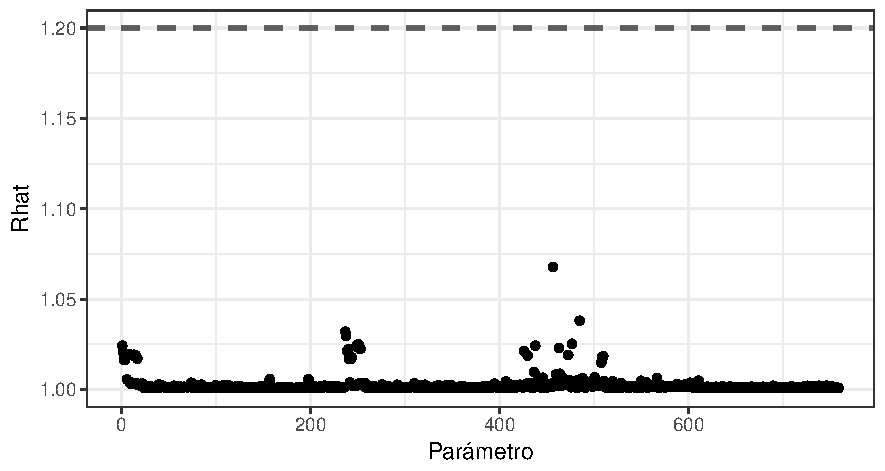
\includegraphics[width=0.9\textwidth]{images/three_levels_r_statistic_params.pdf}
    \caption{Estadística de convergencia $\hat{R}$ de Gelman y Rubin para cada parámetro del modelo multinivel}
    \label{fig:three_levels_r_statistic_params}
\end{figure}

\begin{figure}[H]
    \centering
    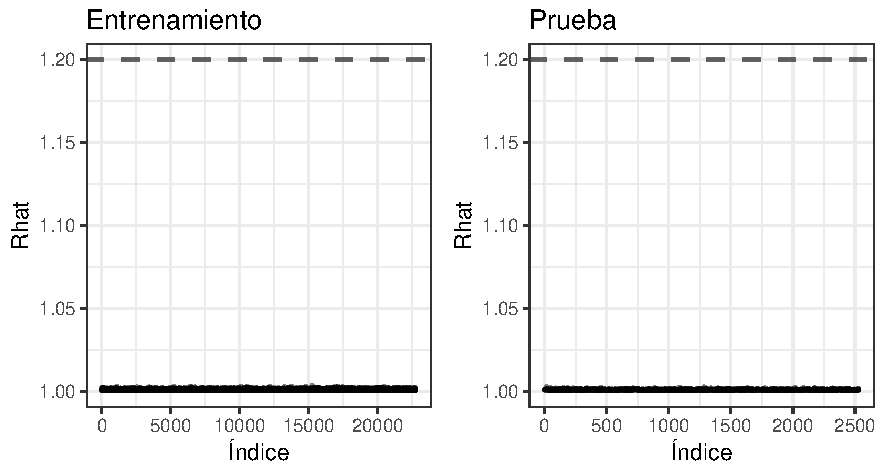
\includegraphics[width=0.9\textwidth]{images/three_levels_r_statistic_yf.pdf}
    \caption{Estadística de convergencia $\hat{R}$ de Gelman y Rubin para estimaciones de la variable respuesta del modelo multinivel}
    \label{fig:three_levels_r_statistic_yf}
\end{figure}

\begin{figure}[H]
    \centering
    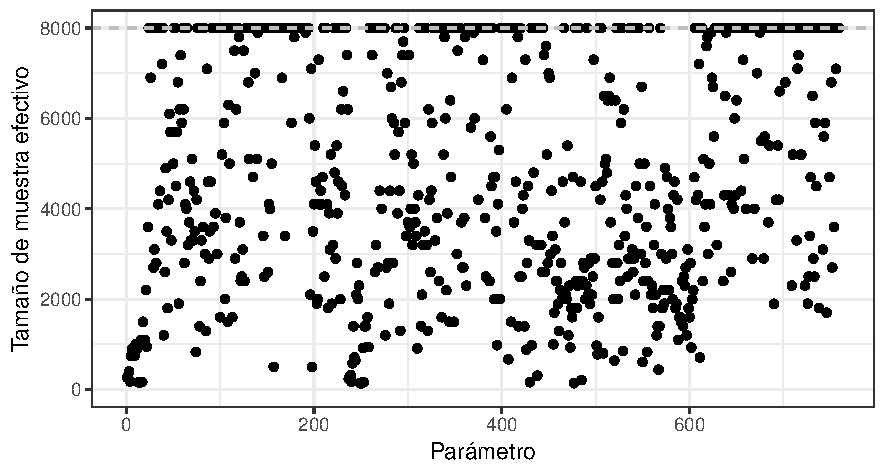
\includegraphics[width=0.9\textwidth]{images/three_levels_n_eff_params.pdf}
    \caption{Tamaño de muestra efectivo para cada parámetro del modelo multinivel}
    \label{fig:three_levels_n_eff_params}
\end{figure}

\begin{figure}[H]
    \centering
    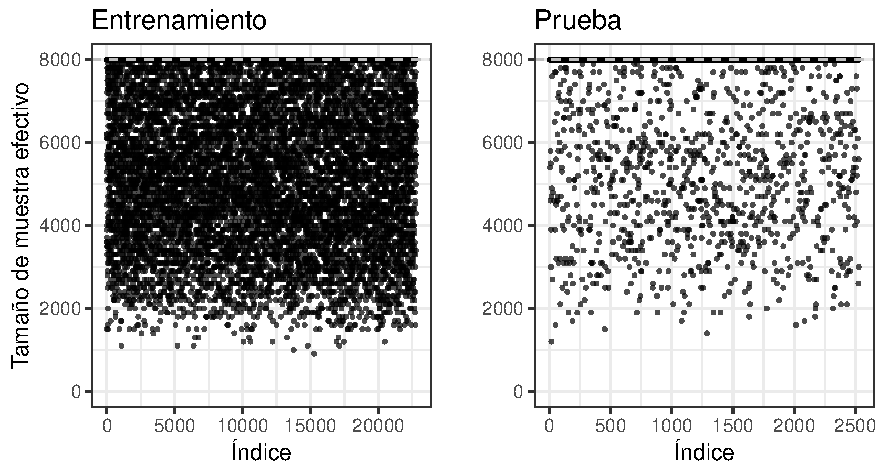
\includegraphics[width=0.9\textwidth]{images/three_levels_n_eff_yf.pdf}
    \caption{Tamaño de muestra efectivo para cada estimación de la variable respuesta del modelo multinivel}
    \label{fig:three_levels_n_eff_yf}
\end{figure}